\section{GPU}
\subsection{GPU란}
GPU 란 Graphics Processing Unit 의 약자로서 원래 2D, 3D 그래픽을 화면에 띄우는 등의
목적으로 만들어졌다. 이전까지는 주로 CPU 를 이용하여 3D 그래픽을 처리하였으나, 더
좋은 그래픽에 대한 수요가 높아짐에 따라 더 빠른 그래픽 처리가 필요했고, 1999 년
NVIDIA 사에서 GeForce256 을 세계 최초의 GPU 라고 판매하면서 ‘GPU’라는 명칭이
사용되었다. 그리고 아래에 서술될 GPU 의 특징으로, 그래픽 처리 뿐만 아니라 대규모 병렬
프로그래밍이 필요한 곳에 많이 쓰이게 되었는데, 이를 일반목적용 컴퓨팅(general-purpose 
computing using a GPU: GPGPU)라고 한다\cite{william2018comsys}. GPGPU 가 처음 지원된 것은 Nvidia GeForce 8800 GTX 부터였다.
\subsection{AI에서 GPU를 쓰는 이유}
CPU 는 순차적인 처리에 특화되어 있어, 제어회로와 캐시메모리가 CPU 면적의 대부분을
차지한다. 그러나 GPU 는 행렬연산과 부동소수점 연산에 특화된 코어 수천개가 대부분을
차지한다. GPU 는 CPU 의 기능 인 순서에 따른 실행, 분기예측, 데이터헤저드 등을 고려하지
않는다. 왜냐하면 모니터에 보여지는 화면의 단위인 픽셀을 계산하는데 한 픽셀이 다른
픽셀에 종속적이지 않기 때문이다.

따라서 GPU 는 단순히 많은 양의 데이터에 대하여 동일한 명령을 동시에 여러 개를
수행하여 여러 개의 데이터를 산출한다. 이를 SIMD(Single Instruction Multi Data)라고 한다.
따라서 GPU 는 동세대 CPU 보다 더 빠른 부동소수점 처리를 보여준다\cite{nvidia2009opencl}.

또한 더 빠른 행렬 연산을 할 수 있는데 \figureautorefname{\ref{fig1}} 에서 1000x1000 행렬곱을 T4 GPU 는 Xeon CPU 보다
약 10 배 더 빠르게 처리할 수 있다. \cite{elice2022gpu}. 이는 합성곱 신경망(Convolutional Neural 
Network, CNN)을 더 빨리 처리하게 해준다. 예를 들어 약 5800 만개의 파라미터를 가지고
있는 약 10000 개의 256x256 이미지를 10 번 학습(10 epochs)하는데 AMD Ryzen 2700x CPU 는
4787 초가 걸렸지만 Nvidia RTX 2080 에서는 745 초가 걸렸다\cite{datamadness2019tensor}.
\begin{figure}[!htb]
  \centering
  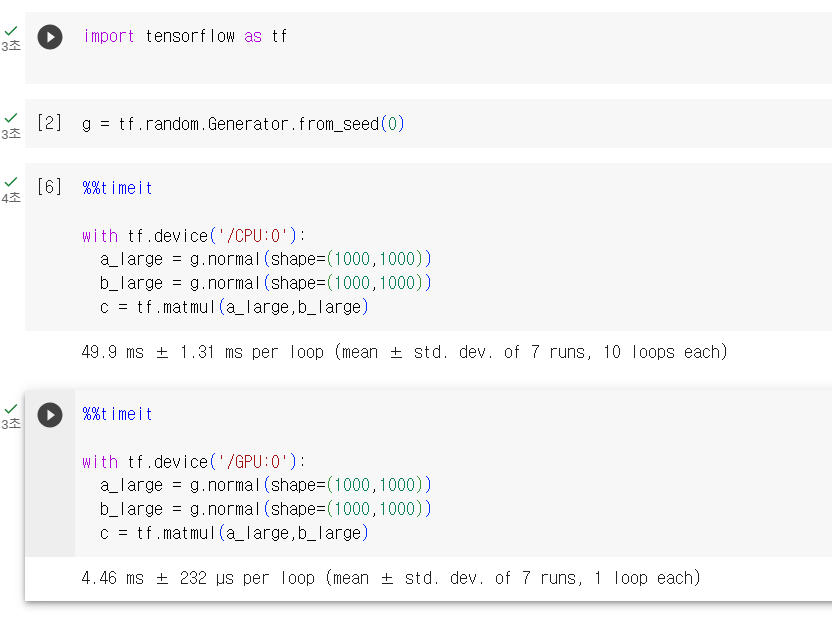
\includegraphics[width=.9\textwidth]{figz/fig1.PNG}
  \caption{행렬곱에서 CPU 와 GPU 의 성능차이: CPU 에서는 루프 당 49.9ms 가 걸렸고,
GPU 에서는 4.46ms 가 걸렸다.}
  \label{fig1}
\end{figure}

\subsection{CUDA 와 스트리밍 다중 프로세서}
GPU 의 대표 회사인 Nvidia 는 미국의 반도체 회사로, GPU 시장 점유율 80\% 안팎으로
예측되고 있다\cite{yonhap2023data}. Nvidia 에서는 GPU 를 GPGPU 로 활용하기 위해 필요한 CUDA 를
개발하였고, GPU 를 병렬 연산에 특화된 수천개의 CUDA 코어로 구성 시켰다.

CUDA(compute Unified Device Architecture)는 GPU 에서 수행하는 알고리즘을 C 
프로그래밍 언어 등으로 개발할 수 있도록 하는 GPGPU 기술이다. CUDA 에서, GPU 에서
실행될 병렬 코드를 커널이라고 부르고, 스레드는 이 커널 함수 중의 한 인스턴스이다.
스레드는 블록으로 묶어지며 이 블록이 스트리밍 다중 프로세서 중 한 개에 할당된다.

스트리밍 다중 프로세서(Streaming multiprocessors)는 레지스터 파일, L1 Cache, CUDA코어,
SFU(Special Functional Units), 이중 왑 스케줄러(Dual warp scheduler) 등으로 구성되어 있다.
SFU 는 코사인,사인, 제곱근과 같은 초월 연산을 수행한다. 이중 왑 스케줄러는 할당받은
블록을 왑(warp, 순차적인 ID 를 가지는 스레드 여러 개를 묶음)으로 나누어 CUDA 코어,
SFU 에 할당한다. CUDA 코어는 Fermi 아키텍처를 기준으로, 두 개의 분리된 파이프라인을
가지고 있다. 하나는 32 비트,64 비트 그리고 그 이상의 정수와 논리/비트 별 연산을 위한 INT 
unit 이고, 다른 하나는 단일 정밀도(single-precision) 부동소수점 연산을 할 수 있는 FP 
unit 이다\cite{william2018comsys}.

그리고 Volta 아키텍처부터 텐서 코어라는 것이 추가되었다. 텐서코어는 AI 에 필요한
행렬 연산에 특화된 부동소수점 연산 장치이다. 텐서 코어는 한 사이클에 4x4 행렬을 한번
곱하고 한번 더하는 연산, 정확히는, 16bit 부동소수점 행렬 2 개를 곱하고, 32bit 부동소수점
행렬 하나를 더하는 연산을 여러 번(2017 년 기준으로 64 번) 할 수 있다. 텐서 코어는 쿠다
코어에 비해 512x512 matrix GEMM(행렬을 한번 곱하고 더하는 연산\cite{nvidia2023matrix})연산 기준으로
약 4 배, 4096x 4096 GEMM 연산 기준으로 약 9 배 더 많은 성능을 제공한다\cite{nvidia2017tensor}. 그러나
실제로 딥러닝에서 활용할 때는, 텐서 코어에 적합하게 데이터를 바꾸는 오버헤드로 인해,
실제 성능 향상은 그보다 낮다고 한다\cite{park2020gpu}.

스트리밍 다중 프로세서 여러 개(아키텍처마다 다르다 Nvidia 의 Fermi 의 경우
16 개이다)와 L2 cache, Giga thread(블록을 스트리밍 다중 프로세서에 할당한다)등이 모여
GPU 를 구성하게 된다.
